\documentclass[12pt]{article}
%\usepackage{amsmath}
\usepackage{graphicx}
\usepackage{listings}
\usepackage{csquotes}
\usepackage{titlesec}
\MakeOuterQuote{"}
\MakeInnerQuote{´}
%\usepackage{enumerate}
\usepackage{natbib} %comment out if you do not have the package
\usepackage{url} % not crucial - just used below for the URL 

%\pdfminorversion=4
% NOTE: To produce blinded version, replace "0" with "1" below.
\newcommand{\blind}{0}

% DON'T change margins - should be 1 inch all around.
\addtolength{\oddsidemargin}{-.5in}%
\addtolength{\evensidemargin}{-1in}%
\addtolength{\textwidth}{1in}%
\addtolength{\textheight}{1.7in}%
\addtolength{\topmargin}{-1in}%


\begin{document}

%\bibliographystyle{natbib}

\def\spacingset#1{\renewcommand{\baselinestretch}%
{#1}\small\normalsize} \spacingset{1}


%%%%%%%%%%%%%%%%%%%%%%%%%%%%%%%%%%%%%%%%%%%%%%%%%%%%%%%%%%%%%%%%%%%%%%%%%%%%%%

\if0\blind
{
  \title{\bf Java Assignemtn CIS 1100}
  \author{Neil Bugeja 51000L
    \\Circular Queue Implementation
    \\Year 1, September Session\bigskip \bigskip}
  \maketitle
} \fi

\if1\blind
{
  \bigskip
  \bigskip
  \bigskip
  \begin{center}
    {\LARGE\bf Title}
\end{center}
  \medskip
} \fi

\bigskip


\newpage
\spacingset{1.8} % DON'T change the spacing!

%-------------------------------
%	CONTENTS
%-------------------------------
\section{AnyClass class}
The class \emph{´AnyClass´} is declared to only contain the integer \emph{´seqNo´}. Getters and setters are created in order to retrieve and set said \emph{´seqNo´}. As per the assignment specifications, three polymorphic methods were created. The first is method \emph{´String getData()´}, which simply returns the value of ´\emph{seqNo}´. The second method is ´\emph{String getKey()}´, and seeing how ´\emph{seqNo}´ is to be returned as a string, ´\emph{String.valueof()}´ was used to fulfil this requirement. Finally, it was stated that for ´\emph{AnyClass}´, the method ´\emph{edit()}´ should be left empty.
\bigskip

\section{Node.java}
Class ´\emph{Node.java}´ has two constructors, one which only consists of ´\emph{AnyClass data}´ and another which adds '\emph{Node next}' to the first.Two methods were created called ´\emph{getNext()}´ and ´\emph{setNext()}´. These getters and setters are vital in the below class ´\emph{CQueue.java}´ as they will set the structure for the queue. Another two methods ´\emph{AnyClass getData()}´ and ´\emph{void setData(AnyClass data)}´ are declared. These methods are used to both get and set the data inside the nodes. Finally, a method show is created to print the data inside the node.
\bigskip

\section{Heterogeneous Circular Queue - CQueue.java}
\bigskip

\subsection{Construction of CQueue}
In this section a circular queue of size 20 nodes must be created. An integer called \emph{´CIRCULAR\_QUEUE\_SIZE´} is created and given the value 20. This is done so that the queue's size is stored in one location and should it need to be changed this can easily be done. \\
\\Firstly, in the \emph{´Node class´}, two methods were created called ´\emph{getNext}´ and ´\emph{setNext}´. These getters and setters are used below to enable the program to both get and set the pointer of the node it is given.\\
\\Secondly, a for loop is created that repeats for \emph{´CIRCULAR\_QUEUE\_SIZE´} times. In every iteration of this loop a new node is created with value null. To create this new node a method 'addNode' is created. \emph{´addNode´} will first check whether the root is null or not. If the root is indead null, this means that the node to be implemented is the first and therefore must be classified as being the root. However, if this is not the case, the root's next will change to point towards the current node, and the current node's next will change to point towards the root. The loop will traverse the queue until it reaches the last node, guaranteeing that the queue will be circular.\\
\\The below diagram may help better illustrate what was explained above:
%Image:
\begin{figure}[h]
\centering
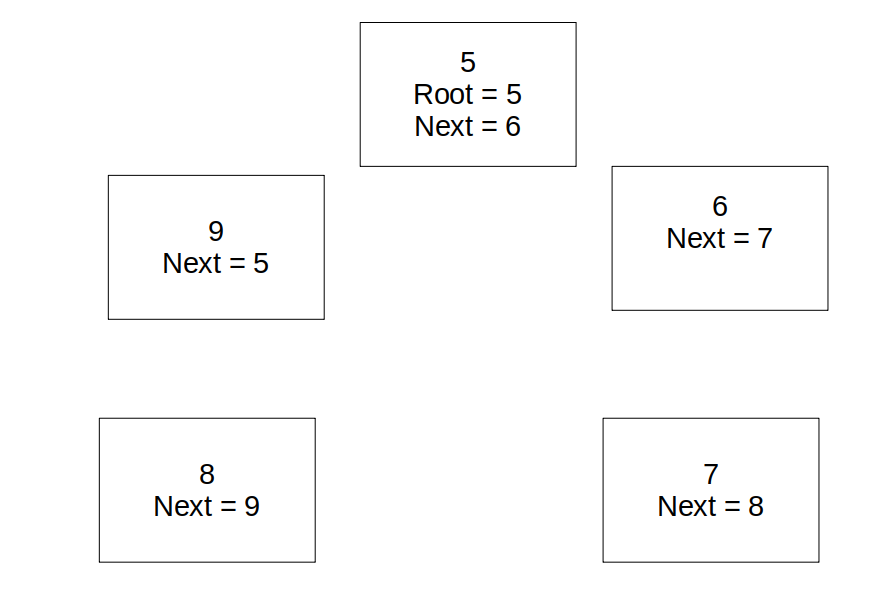
\includegraphics[scale=0.30]{Images/Insert.png}
\end{figure}
\bigskip


By the means of the ´\emph{addNode}´ method, a circular queue is successfully created of size \emph{´CIRCULAR\_QUEUE\_SIZE´}.
\bigskip

\subsection{Method boolean put(AnyClass newObj)}
This method makes use of the same principles and ideas used to create the queue itself. Firstly, in the \emph{´node class´} two methods are created which will be used to get data from a node and set data to a node.\\
\\Secondly, in the \emph{´CQueue class´}, the method ´\emph{put}´ is created. Like the method ´\emph{addNode}´, it will first check if the root of the queue is null. If this is the case, the root is simply filled with data by using the setter. However, if the root is not null the program will traverse the queue as it has done in the previous method to create the nodes, but this time while it is visiting a node it will set data into it.\\
\\If neither of these cases are met the method will return false, indicating that the queue is full.
\bigskip

\subsection{AnyClass serve()}
This method will first check whether or not the queue is empty. If the queue is empty it simply only returns that there is no content available. Otherwise, the method will grab the first object and give it the value of the one next to it. This process will repeat until the entire queue has been through this process. After this has been done, the object which was previously second in the queue is now the root.The image below will help illustrate the explanation given.\\
\\
\begin{figure}[h]
\centering
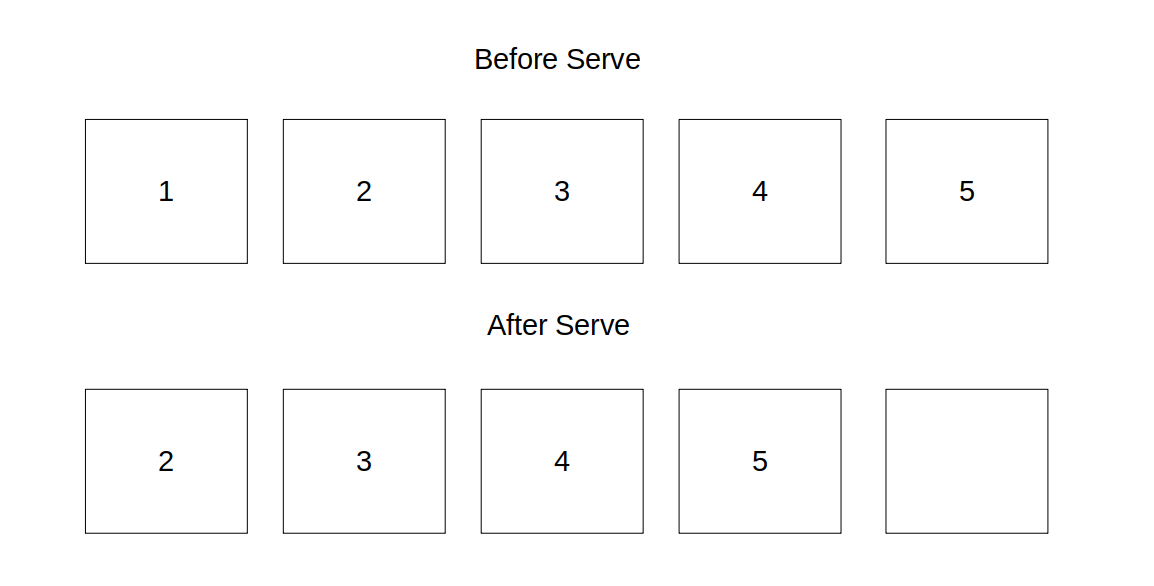
\includegraphics[scale=0.30]{Images/serve.png}
\end{figure}
\bigskip

\subsection{void listAll()}
To list all the data in the circular queue, this method will traverse the queue by the same method that it has been doing previosly. The only difference is that every time a node filled with data is encountered, the data is acquired and outputted for the user to see. By the end of the method all the data in the queue will be displayed.\\


\subsection{AnyClass editObject(String key)}
This method will once again begin by traversing the entire queue. If it encounters an array with data it will check to see if it matches with the key given. If this is the case, the key's data is acquired and used in the method \emph{´edit´} found in Employee.java. 

\subsection{void changePayOfAll(int percent)}
This method traverses the entire queue and in each instance where data is encountered, the object is passed through to the method ´\emph{editAll(int percentage)}´. This method is declared in the ´\emph{AnyClass}´ class and is later overridden in the ´\emph{Employee}´ class. In the ´\emph{Employee}´ class, the method ´\emph{editAll(int percentage)}´ will set the salary to a new salary. To calculate the new salary, the integer percentage must be transformed into a type double.
\bigskip

%------------------------------------------------

\section{Emplyee - Employee.java}

When declaring an employee, the following must be assigned:
\\
\\1. A number relating to the sequence number
\\2. The employee's surname
\\3. The employee's salary which is declared as a double.\\
\\The class has the appropriate getters and setters in place to get and set salary and get the employee's key which is the surname. A method is also created which retrieves the employee's data which includes his id number, surname(key), and salary.\\
\\Lastly, two methods are created. One is used to edit the employee's salary. This method will first display's the employee's current salary by means of the getter, and later set a new salary by means of a setter. The other method is the ´\emph{editAll()}´ method which has been explained in the previous section.
\bigskip 

%------------------------------------------------
\section{PartTimer - PartTimer.java}
PartTimer extends employee as it is basically employee but with a few additions. A constructor for PartTimer is present as hours must also be declared in the case for a part time employee. The constructor makes use of supers as they are the same as ´\emph{Employee.java}´. A method is present which retrieves the partTimer's hours and another method ´\emph{getData()}´ which overrides the method ´\emph{getData()}´ found in ´\emph{Employee.java}´. This is important as without it the partTimer's hours cannot be viewed.
\bigskip

\section{Deliverables - Main.java}
The menu starts by first creating the ´\emph{CQueue}´ which will be used to store both types of employees. Next, the menu is displayed, giving the user a variety of options. Depending on the option chosen, a switch is present to employ the method corresponding with the user's request.\\
\\Below is a list of all options and an explanation on how they function:

\subsection{Populate Queue}
The queue must be populated with both full time and part time employees. Therefore, the method will first ask the user how many new full time employees have to be inserted. In the case of full time employees the sequence number, surname and salary are required. Next, the program will ask the user how much part time employees must be created. The same credentials as employee must be given along with the addition of hours worked. The employees are inserted into the queue by means of the ´\emph{put}´ method developed earlier.

\subsection{List all objects in queue}
This method simply calls the method ´\emph{listAll()}´ developed in the ´\emph{CQueue}´ section of this program.

\subsection{Search for Employee}
To fulfil this requirement, first a method of type ´\emph{AnyClass}´ called ´\emph{listEmployee}´ was created in the ´\emph{CQueue}´ class. This method requires a String '\emph{key}' and an int ´\emph{seqNo}´. These variables are the variables that the user will input and used to search the queue with. With that said, the method will traverse the entire queue and search for an objects which matches the user's ´\emph{seqNo}´ and ´\emph{key}´. Care was taken for the searching to not be case sensitive. Should an object with matching credentials be found, the method will output said object. Else nothing will happen.

\subsection{Update Payment of a single Employee}
To complete this task, the method ´\emph{editObject}´ which was previously created is used. In this section, the method simply asks the user for the employee's surname(key) which needs to be edited, and said surname is inserted into the method ´\emph{editObject()}´. This method works fine, however should the queue contain two or more objects with the same surname, the user must edit all salary values. The same procedure used in ´Search for employee´ where both sequence number and surname must be entered cannot be used as that would violate the requirements placed in the method ´\emph{editObject()}´ in which only a String key must be entered in it's parameters.

\subsection{Update payment of all persons by percentage}
This method enters the user's chosen percentage change into the method ´\emph{changePayOfAll()}´ in which the necessary adjustments will be made to all employee's salaries. After this, the list of all employees along with their salaries is displayed, to show the user of all the changes made. This method will also work with negative numbers, should the user wish to decrease the employee's salary.

\subsection{Present and delete first item in queue (SERVE)}
This method is present to make use of the serve method developed earlier in the 'CQueue' class.

\bigskip
%------------------------------------------------
\newpage
\section{Source Code}
\bigskip

\footnotesize
\subsection{Package dataobjects}
\subsubsection{AnyClass.java}
\begin{lstlisting}
package dataobjects;

public class AnyClass{

    public int seqNo;

    public AnyClass(int seqNo){
        this.seqNo = seqNo;
    }

    public int getSeqNo(){
        return seqNo;
    }

    public void setSeqNo(int seqNo){
        this.seqNo = seqNo;
    }

    public String getData(){
        return "Sequence number: "+seqNo;
    }

    public String getKey(){
        return String.valueOf(seqNo);
    }

    public void edit(){
    }

    public void editAll(int percentage){

    }

}
\end{lstlisting}

\subsubsection{Employee.java}
\begin{lstlisting}
package dataobjects;
import java.util.Scanner;

public class Employee extends AnyClass{
    String surname;
    double salary;

    public Employee (int num, String surname, double salary) {
        
        super (num);
        this.surname = surname;
        this.salary = salary;        
    }

    public double getSalary(){
        return salary;
    }

    public double setSalary(double salary){
        this.salary = salary;
        return salary;
    }

    public String getData(){
        return super.getData() + "\nEmployee:        " +surname+ "\nSalary:          " + getSalary() +"\n";
    }

    public String getKey(){
        return surname;
    }

    public void edit(){
        Scanner in = new Scanner(System.in);
        System.out.println("Current Salary:" +getSalary());
        System.out.println("Enter new salary: ");
        double newSalary = in.nextDouble();   
        setSalary(newSalary);    
    }

    public void editAll(int percentage){
        double perc = percentage;
        double newSalary = getSalary()*(1+(perc/100));
        setSalary(newSalary);
    }
}

\end{lstlisting}

\subsubsection{PartTimer.java}
\begin{lstlisting}
package dataobjects;

public class PartTimer extends Employee{

    int hours;

    public PartTimer (int num, String surname, double pay, int hours) {
        
        super (num, surname, pay);
        this.hours = hours;      
    }

    public int getHours(){
        return hours;
    }

    public String getData(){
        return "Sequence number: "+getSeqNo() + "\nEmployee:        " +surname+ "\nSalary:          " + getSalary() +"\n" +"Hours:           "+getHours()+"\n";
    }
}

\end{lstlisting}

\newpage
\subsection{Package linearnode}

\subsubsection{Node.java}
\begin{lstlisting}
package linearnodes;
import dataobjects.*;

public class Node {
    private Node next;
    private AnyClass data;

    public Node(AnyClass data){
        this.data = data;
    }

    public Node(Node next, AnyClass data){
        this.next = next;
        this.data = data;
    }

    //Used for node pointers
    public Node getNext() {
        return next;
    }

    //Used for node pointers
    public void setNext(Node next) {
        this.next = next;
    }

    //Used for node data
    public AnyClass getData() {
        return data;
    }

    //Used for node data
    public void setData(AnyClass data) {
        this.data = data;
    }

    public void show(){
        System.out.println(data.getData());
    }
}

\end{lstlisting}
\newpage
\subsection{Package linearstructures}

\subsection{CQueue.java}
\begin{lstlisting}
package linearstructures;
import dataobjects.*;
import linearnodes.*;


public class CQueue {
    //declare queue size & set root to null
    private final int CIRCULAR_QUEUE_SIZE = 20;
    private Node root = null;

    public CQueue(){
        //create circular list with previously declared size
        for(int i=0; i<CIRCULAR_QUEUE_SIZE+1; i++){
            addNode(new Node(null));
        }
    }

    public void addNode(Node node){       
        if(root == null){
            root = node;
            node.setNext(root);
        }else{
            //Traverse until arrives at the last node
            Node n = root;
            while(n.getNext()!=root){
                n = n.getNext();
            }
            node.setNext(root);
            n.setNext(node);
        }        
    }

    public boolean put(AnyClass newObj){
        if(root.getData()==null){
            root.setData(newObj);
            return true;
        }
        Node n = root;
        while(n.getNext()!=root){
            n = n.getNext();
            if(n.getData()==null){
                n.setData(newObj);
                return true;
            }
        }
        return false;        
    }

    public AnyClass serve(){
        Node n = root;

        //If empty
        if(root.getData() == null){
            System.out.println("List is empty");
            return null;
        }else{
            System.out.println("Subject deleted: ");
            System.out.println("");
            root.show();
            while(n.getNext()!=root){
                //gives each node the value of the node infront of it.
                n.setData(n.getNext().getData());
                n = n.getNext(); 
            }
        }

        return null;
    }   

    public AnyClass listEmployee(String key, int seqNo){
        Node n = root;
        while(n.getNext()!=root){
            if(n.getData()!=null){
                if(n.getData().getKey().equalsIgnoreCase(key) && n.getData().getSeqNo() == seqNo){                   
                    n.show();             
                }
            }
            n = n.getNext();
        }
        return null; //not found
    }

    public void listAll(){
        Node n = root;
        while(n.getNext()!=root){
            if(n.getData()!=null){
                n.show();
            }
            n = n.getNext();
        }
    }

    public AnyClass editObject(String key){
        Node n = root;
        while(n.getNext()!=root){
            if(n.getData()!=null){
                if(n.getData().getKey().equalsIgnoreCase(key)){                   
                    n.getData().edit();                 
                }
            }
            n = n.getNext();
        }
        return null; //not found
    }

    public AnyClass changePayOfAll(int percentage){
        Node n = root;
        while(n.getNext()!=root){
            if(n.getData()!=null){
                n.getData().editAll(percentage);
            }
            n = n.getNext();
        }
        return null; //not found
    }
}//end class

\end{lstlisting}
\newpage
\subsection{Main.java}
\begin{lstlisting}
import dataobjects.*;
import linearstructures.*;
import java.util.Scanner;

public class Main {
    public static void main(String args[]) {        
        menu();
    }

    public static void menu(){
        CQueue myQueue = new CQueue();
        int choice;
        Scanner in = new Scanner(System.in);
        do{
            System.out.println("Please enter your selection:");
            System.out.println("1. Populate queue");            
            System.out.println("2. List all object in queue");
            System.out.println("3. Search for employee");
            System.out.println("4. Update payment of a single person");
            System.out.println("5. Update payment of all persons by percentage");
            System.out.println("6. Present and delete first item in queue (SERVE)");
            System.out.println("7. Generate List");
            System.out.println("8. Exit");

            choice = in.nextInt();

            switch(choice){
                case 1: populateQueue(myQueue);
                    break;
                case 2: listAll(myQueue);
                    break;   
                case 3: searchEmployee(myQueue);
                    break; 
                case 4: updateEmployeePayment(myQueue);
                    break;
                case 5: updateAll(myQueue);
                    break; 
                case 6: serve(myQueue);
                    break;   
                case 7: generateList(myQueue);
                    break;            
            }
        }while(choice!=8);
    }

    public static void populateQueue(CQueue myQueue){
        Scanner in = new Scanner(System.in);
        int seqNo;
        String surname;
        double salary = 0;
        int hours = 0;

        System.out.println("How many new FULL TIME EMPLOYEES: ");
        int n = in.nextInt();
        
        for(int i=0; i<n; i++){
            System.out.print("Enter sequence number:");
            seqNo = in.nextInt();
            System.out.print("Enter employee surname(key): ");
            surname = in.nextLine();
            surname = in.nextLine();
            System.out.print("Enter employee salary: ");
            salary = in.nextDouble();
            System.out.println("");
            myQueue.put(new Employee(seqNo, surname, salary));
        }

        System.out.println("How many new PART TIME EMPLOYEES: ");
        n = in.nextInt();
        
        for(int i=0; i<n; i++){
            System.out.print("Enter sequence number:");
            seqNo = in.nextInt();
            System.out.print("Enter employee surname(key): ");
            surname = in.nextLine();
            surname = in.nextLine();
            System.out.print("Enter employee salary: ");
            salary = in.nextDouble();
            System.out.print("Enter employee hours: ");
            hours = in.nextInt();
            System.out.println("");
            myQueue.put(new PartTimer(seqNo, surname, salary, hours));
        }     
        
    }

    public static void listAll(CQueue myQueue){       
        myQueue.listAll();
    }

    public static void searchEmployee(CQueue myQueue){    
        Scanner in = new Scanner(System.in);
        String userSearch;           
        System.out.println("Enter surname(key): ");
        userSearch = in.nextLine();
        System.out.println("Enter sequence number: ");
        int userNumber = in.nextInt();
        myQueue.listEmployee(userSearch, userNumber);
        System.out.println("");
    }

    public static void updateEmployeePayment(CQueue myQueue){       
        Scanner in = new Scanner(System.in);
        String userSearch;   
        System.out.println("Enter surname(key): ");
        userSearch = in.nextLine();
        myQueue.editObject(userSearch);
        System.out.println("");
    }

    public static void updateAll(CQueue myQueue){  
        Scanner in = new Scanner(System.in);   
        System.out.println("Enter percentage to change payments by: ");
        System.out.println("Example: for 10% increase enter 10");
        System.out.println("Example: for 10% decrease enter -10");
        int user = in.nextInt();
        myQueue.changePayOfAll(user);
        System.out.println("Payment Updated!");
        System.out.println("New list:");
        myQueue.listAll();
    }

    public static void serve(CQueue myQueue){
        myQueue.serve();
    }

    public static void generateList(CQueue myQueue){
        myQueue.put(new Employee(1, "bugeja", 50000));
        myQueue.put(new Employee(2, "sant", 40000));
        myQueue.put(new PartTimer(3, "curmi", 30000, 35));
        myQueue.put(new PartTimer(4, "bocc", 20000, 12));
    }
}

\end{lstlisting}


%------------------------------------------------
\end{document}
